\section{Results}


\subsection{IOS Medical Apps}

\begin{figure}[H]
    \centering
    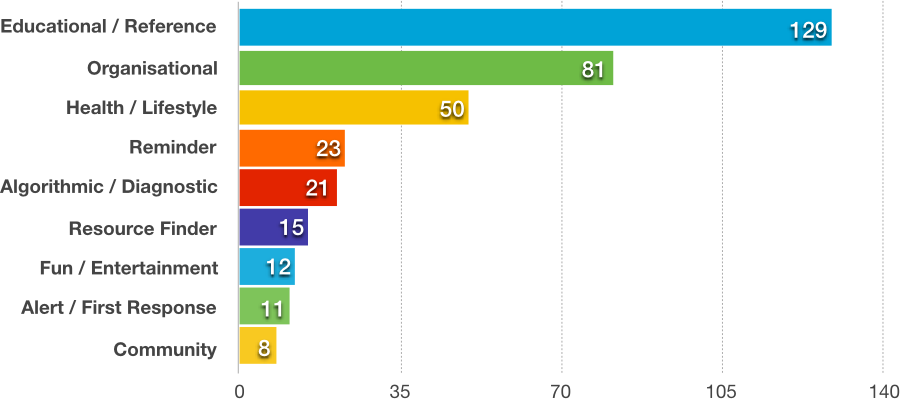
\includegraphics[width=\textwidth]{assets/market_research/apple_chart1.png}
    \caption{Medical Apps on the iTunes Apple Store, Search conducted on 17.05.2016}
    \label{fig:itunes_apps}
\end{figure}


\subsection{Android Medical Apps}

\begin{figure}[H]
    \centering
    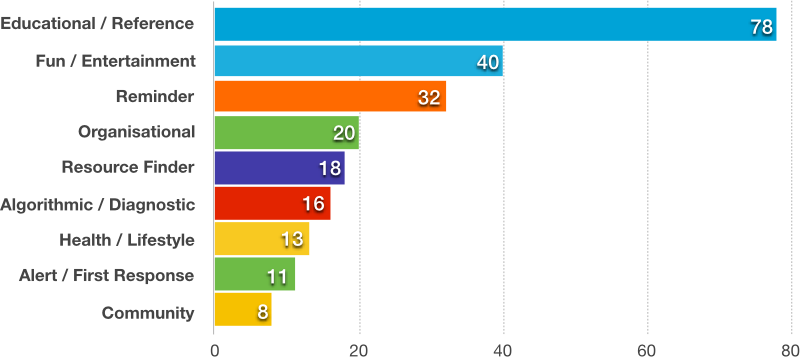
\includegraphics[width=\textwidth]{assets/market_research/android_chart.png}
    \caption{Medical Apps on the Goolge Play Store, Search conducted on 17.05.2016}
    \label{fig:android_apps}
\end{figure}

\subsection{Dermatology Apps 2013 vs 2016}

Mobile apps are an especially good fit for dermatology-related care. Most dermatological conditions are by nature visible. The initial diagnosis and follow up monitoring is mostly done visually. A mobile device with a camera can aid patients and practitioners in the diagnosis of a dermatological condition and tracking it's development. The article Mobile Applications in Dermatology\cite{Brewer_2013} in 2013 identified 229 dermatology-related apps across 5 app platforms ( Android, Apple, Blackberry, Nokia, and Windows ). These were grouped into categories based on their primary functionality. The "Self-surveillance/diagnosis" category was the second largest on the Android and Apple platforms, with 13 and 24 apps respectively.

\begin{figure}[H]
    \centering
    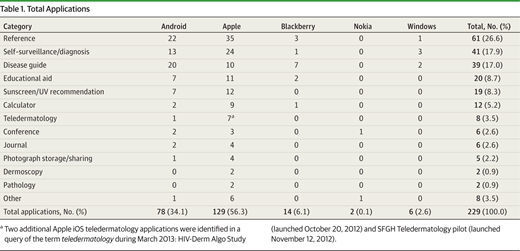
\includegraphics[width=\textwidth]{assets/market_research/brewer.png}
    \caption{Total Applications, Brewer 2013}
    \label{fig:brewer}
\end{figure}

Using the same search criteria and categories from the article above indicates that the availability of dermatological apps is growing. Today there are 33 dermatological apps on the Apple platform that can be identified as having "Self-surveillance/diagnostic" features. With the exception of the "Reference" category, all other categories show significantly higher numbers of available apps.


\begin{figure}[H]
    \centering
    \includegraphics[width=\textwidth]{assets/market_research/apple2013vs1016.png}
    \caption{Demotological Apps by Category, July 2013(Brewer 2013) vs May 2016}
    \label{fig:apps_vs}
\end{figure}

It is important to note that the categories listed above are not defined in the stores. The apps must be manually assigned to a category based on an interpretation of the description text in the store and information obtainable on related websites. It is possible therefore that apps that were originally designated to the “Reference” category might have been interpreted in this paper as a “Educational aid” app for example. The interpretation of the functionality of an app is fuzzy in many cases, and many apps have some crossover functionality. An app developed for self-surveillance will often contain information pertaining to symptoms and treatment ( reference ).